\documentclass[conference]{IEEEtran}
\IEEEoverridecommandlockouts

\usepackage{cite}
\usepackage{amsmath,amssymb,amsfonts,amsthm}
\usepackage{algorithmic}
\usepackage{algorithm}
\usepackage{graphicx}
\usepackage{textcomp}
\usepackage{booktabs}
\usepackage{tabularx}
\usepackage{url}
\usepackage{array}
\usepackage{microtype}
\usepackage{balance}

% Spacing optimizations for strict 8-page budget
\setlength{\textfloatsep}{2.5pt plus 1pt minus 1pt}
\setlength{\floatsep}{2.5pt plus 1pt minus 1pt}
\setlength{\intextsep}{2.5pt plus 1pt minus 1pt}
\setlength{\dbltextfloatsep}{2.5pt plus 1pt minus 1pt}
\setlength{\dblfloatsep}{2.5pt plus 1pt minus 1pt}

% Compact bibliography formatting
\let\oldthebibliography\thebibliography
\renewcommand{\thebibliography}[1]{%
  \oldthebibliography{#1}%
  \setlength{\itemsep}{0pt plus 0.1pt}%
  \setlength{\parskip}{0pt}%
}

\newtheorem{theorem}{Theorem}
\newtheorem{lemma}{Lemma}
\newtheorem{definition}{Definition}
\newtheorem{invariant}{Invariant}

\newcolumntype{Y}{>{\centering\arraybackslash}X}
\graphicspath{{./figures/}}

\begin{document}

\title{SMBFlow: A Deterministically Governed Multi-Agent Architecture for Context-Aware Workflow Automation in Enterprise Environments}

\author{\IEEEauthorblockN{Hemantkumar~S.~Lakhane\IEEEauthorrefmark{1}, Tanmay Kumbhare\IEEEauthorrefmark{1}, Varsha Dange\IEEEauthorrefmark{1}, Dhanashri Khode\IEEEauthorrefmark{1}, and Khushi Ghumre\IEEEauthorrefmark{1}}
\IEEEauthorblockA{\IEEEauthorrefmark{1}Department of Artificial Intelligence and Data Science / Machine Learning \\
Vishwakarma Institute of Technology, Pune, 411037, Maharashtra, India \\
Email: \{hemantkumar.lakhane24, tanmay.kumbhare24, varsha.dange1, dhanashri.khode24, khushi.ghumre24\}@vit.edu}
}

\maketitle

\begin{abstract}
Enterprises increasingly deploy Large Language Model (LLM) multi-agent systems to automate mission-critical workflows across fragmented software ecosystems. However, unconstrained stochastic agents introduce catastrophic failure modes: hallucinated state transitions, unauthorized side-effects, prompt injection vulnerabilities, and absent cryptographic auditability. In this paper, we present \textbf{SMBFlow}, an enterprise-grade multi-agent workflow architecture grounded in a strict principle: \emph{probabilistic agents propose, deterministic gates decide}. SMBFlow enforces capability-based execution isolation where agents hold zero tool credentials, requiring cryptographically signed, single-use HMAC execution tokens issued only after typed policy predicates and calibrated risk scoring are satisfied. We implement conformal risk calibration bounding false executions, adaptive human-in-the-loop (HITL) thresholding, Saga-style backward compensation, hybrid GraphRAG context retrieval combining dense embeddings with Personalized PageRank, and a quality-constrained cost optimizer. Furthermore, SMBFlow hardens execution provenance through a Merkle-tree Evidence and Provenance Infrastructure (EPI) with periodic signed external anchoring, providing formal computational resistance against retroactive tampering and truncation. We conduct an extensive empirical evaluation across three multi-tenant enterprise workflows (900 full runs, 240 adversarial attack vectors, and 1,500 calibration trials). SMBFlow achieves a 0.0\% unsafe execution rate (compared to 14.7\%--20.3\% for ungated ReAct and 8.0\%--8.7\% for LangGraph guardrails), reduces token expenditure by 51.8\% relative to frontier models ($p < 10^{-50}$, Cohen's $d = 10.06$), resists 100\% of adversarial attacks, and verifies 50,000 execution steps in 704.8\,ms while adding merely 2.21\,ms of non-LLM governance overhead.
\end{abstract}

\begin{IEEEkeywords}
Multi-Agent Systems, Workflow Orchestration, Deterministic Governance, Capability Security, Conformal Risk Calibration, GraphRAG, Cryptographic Provenance.
\end{IEEEkeywords}

% =========================================================================
\section{Introduction}
% =========================================================================

Small and medium-sized enterprises (SMEs) face acute operational bottlenecks due to fragmented Software-as-a-Service (SaaS) applications, manual cross-platform data synchronization, and lean technical resources~\cite{weske2019bpm}. While modern businesses rely on diverse platforms---CRM tools, billing gateways, ERP databases, and messaging channels---these systems lack autonomous interoperability. 

Recent advancements in Large Language Model (LLM) agents and multi-agent architectures~\cite{yao2023react, schick2023toolformer, wu2023autogen, langgraph2024, hong2024metagpt, wang2024agentsurvey, xi2023rise} offer substantial promise for enterprise workflow automation. By decomposing complex workflows into specialized agent personas, multi-agent frameworks parse unstructured business documents, reason across relational records, and formulate multi-step operational plans.

However, deploying unconstrained stochastic agents in production enterprise environments introduces prohibitive risks: (1) \textbf{Stochastic State Mutation}: Generative LLMs exhibit probabilistic drift and hallucination, generating invalid tool parameters (e.g., erroneous ledger modifications or unauthorized refunds)~\cite{ruan2024toolemu}; (2) \textbf{Prompt Injection}: Indirect prompt injections embedded in external data (e.g., invoices, emails) hijack agent reasoning, leaking tenant data or evading safety prompts~\cite{greshake2023promptinjection, perez2022ignore}; (3) \textbf{Credential Over-Privilege}: Conventional frameworks equip agent personas with ambient API keys, enabling compromised agents to execute external side effects directly~\cite{qin2024toolllm}; (4) \textbf{Absence of Cryptographic Provenance}: Existing frameworks log state mutations into mutable tables without cryptographic integrity proofs, failing regulatory compliance standards (e.g., EU AI Act~\cite{euai2024}) requiring tamper-evident lineage~\cite{crosby2009tamper, moreau2013prov}; (5) \textbf{Prohibitive Operational Expenditure}: Universal routing to frontier models incurs unsustainable inference expenses~\cite{chen2023frugalgpt, ong2024routellm}.

To resolve these fundamental challenges, we introduce \textbf{SMBFlow}, an enterprise-grade multi-agent workflow architecture grounded in a strict systems invariant: \emph{probabilistic LLM agents propose actions, but deterministic policy engines and cryptographic execution gates decide and execute}.

\textbf{Contributions}: The core contributions of this work are:
\begin{itemize}\setlength{\itemsep}{0pt}\setlength{\parskip}{0pt}
    \item \textbf{Capability-Based Execution Isolation}: We design an execution plane where agents possess zero tool credentials. External connectors accept invocations if and only if accompanied by a single-use, HMAC-signed execution token issued exclusively by a deterministic governance gate after static policy checking and risk verification. We formally state and prove the execution isolation invariant.
    \item \textbf{Calibrated Risk Scoring and Adaptive HITL}: We replace heuristic risk weights with Platt-calibrated scoring bounded by conformal false-execute limits ($\le 5\%$), paired with an online adaptive Human-in-the-Loop (HITL) threshold controller that reduces operator review load while maintaining safety.
    \item \textbf{Hardened Merkle Provenance (EPI)}: We construct an Evidence and Provenance Infrastructure (EPI) combining Merkle-tree batching with signed external checkpoint anchoring. We formally prove computational immutability under collision resistance (Theorem~1) and truncation detection under external anchoring (Theorem~2).
    \item \textbf{Hybrid GraphRAG and Constrained Routing}: We formulate a multi-hop context retrieval engine fusing dense vector similarity with Personalized PageRank (PPR), alongside a quality-constrained cost optimizer reducing inference expenditure by 51.8\% ($p < 10^{-50}$).
    \item \textbf{Comprehensive Empirical Validation}: We construct a reproducible testbed spanning three multi-tenant enterprise workflows (900 full runs, 240 red-team attack vectors, 1,500 calibration trials). We measure latency, cost, safety, scalability to 100 concurrent tenants, and verification scaling to 50,000 steps.
\end{itemize}

% =========================================================================
\section{Related Work and Gap Analysis}
% =========================================================================

\subsection{Multi-Agent Frameworks and Tool-Use Safety}
Autonomous LLM agents leverage cognitive paradigms such as ReAct~\cite{yao2023react} and Toolformer~\cite{schick2023toolformer} to interleave reasoning with tool execution. Multi-agent systems such as AutoGen~\cite{wu2023autogen}, MetaGPT~\cite{hong2024metagpt}, and Generative Agents~\cite{park2023generative} coordinate agents via natural language dialogue. LangGraph~\cite{langgraph2024} introduces cyclic state-graph scheduling. However, as demonstrated by ToolEmu~\cite{ruan2024toolemu}, conversational multi-agent systems suffer from cascading hallucination and lack deterministic execution containment. Prompt-level guardrails (e.g., Llama Guard~\cite{inan2023llamaguard}, NeMo Guardrails~\cite{rebedea2023nemoguardrails}) remain susceptible to adversarial circumvention and indirect injection~\cite{greshake2023promptinjection, robey2023smoothllm}. SMBFlow departs from prompt-level filtering by enforcing out-of-band deterministic policy validation over schema-typed action proposals.

\subsection{Workflow Management and Transactional Sagas}
Industrial workflow engines such as Apache Airflow~\cite{airflow2019} and Temporal~\cite{temporal2022} orchestrate deterministic Directed Acyclic Graphs (DAGs) with robust state recovery~\cite{vanderAalst2016process, weske2019bpm}. However, traditional BPMS lack generative reasoning capabilities required to parse ambiguous enterprise documents. Furthermore, distributed transactions in heterogeneous environments require compensating actions, formalized by Garcia-Molina and Salem's Saga pattern~\cite{garciamolina1987sagas}. SMBFlow integrates Saga-style backward compensation into agent orchestration, guaranteeing automated rollback upon mid-workflow failure or human rejection~\cite{amershi2019guidelines, holzinger2016hitl}.

\subsection{Cryptographic Logging and Model Cascades}
Tamper-evident logging originates from Merkle trees~\cite{merkle1987signature} and authenticated log structures~\cite{crosby2009tamper, laurie2014ct}. W3C PROV~\cite{moreau2013prov} defines provenance ontologies, but standard agent architectures log execution steps in mutable application databases without cryptographic integrity proofs. In inference optimization, FrugalGPT~\cite{chen2023frugalgpt} and RouteLLM~\cite{ong2024routellm} demonstrate model cascades and learned routers that select compact models for routine tasks. SMBFlow formulates model routing as a constrained integer program, enforcing stage-specific quality guarantees. Table~\ref{tab:related_work} synthesizes the architectural gap between SMBFlow and existing systems.

\begin{table}[t]
\caption{Architectural and Governance Comparison Against Existing Frameworks}
\label{tab:related_work}
\centering
\scriptsize
\setlength{\tabcolsep}{2.5pt}
\begin{tabularx}{\linewidth}{l X X X X}
\toprule
\textbf{Architectural Feature} & \textbf{AutoGen}~\cite{wu2023autogen} & \textbf{LangGraph}~\cite{langgraph2024} & \textbf{Temporal}~\cite{temporal2022} & \textbf{SMBFlow} \\
\midrule
Cognitive LLM Reasoning & Yes & Yes & No & \textbf{Yes} \\
Deterministic DAG Engine & No & Partial & Yes & \textbf{Yes} \\
Capability Token Isolation & No & No & No & \textbf{Yes (HMAC)} \\
Typed Schema Policy DSL & No & Prompt-only & No & \textbf{Yes (Static)} \\
Conformal Risk Calibration & No & No & No & \textbf{Yes ($\le 5\%$)} \\
Adaptive HITL Escalation & No & Static & Manual & \textbf{Yes (Online)} \\
Saga-Style Compensation & No & No & Yes & \textbf{Yes (100\%)} \\
Hybrid GraphRAG (PPR) & No & No & No & \textbf{Yes ($\alpha=0.6$)} \\
Merkle EPI + Anchor Checkpoint & No & No & No & \textbf{Yes (SHA-256)} \\
Quality-Constrained Routing & No & No & No & \textbf{Yes ($-51.8\%$)} \\
\bottomrule
\end{tabularx}
\end{table}

% =========================================================================
\section{Threat Model and Problem Formulation}
% =========================================================================

\subsection{Threat Model and Security Assumptions}
\textbf{Assets}: Protected assets comprise: (i) tenant execution state and relational databases; (ii) external tool connectors (e.g., payment gateways, CRM APIs, corporate email); (iii) confidential tenant context; and (iv) immutable execution audit logs.

\textbf{Adversary Capabilities}: We consider an adversary capable of: (i) injecting indirect adversarial prompts into untrusted external data sources ingested during retrieval; (ii) inducing stochastic agent hallucinations leading to malformed arguments, out-of-policy spending, or unauthorized recipients; (iii) compromising an LLM agent persona to emit arbitrary action proposals attempting cross-tenant data access; (iv) retroactively modifying, deleting, reordering, or truncating execution records stored in the audit persistence layer.

\textbf{Security Assumptions}: Cryptographic primitives (HMAC-SHA256, digital signatures) are computationally secure against polynomial-time adversaries. The Governance Gate and Key Management Service (KMS) run within a trusted execution boundary. Physical hardware attacks and zero-day OS exploits are out of scope.

\subsection{Problem Formulation}
An enterprise workflow is formulated as a directed graph $\mathcal{W} = \langle \mathcal{V}, \mathcal{E}, \mathcal{T}, \mathcal{P} \rangle$, where $\mathcal{V} = \{v_1, \dots, v_n\}$ represents agent nodes, $\mathcal{E}$ denotes dependencies, $\mathcal{T}$ represents tenant context, and $\mathcal{P}$ is the active policy set. At node $v_k$, an agent generates an action proposal:
\begin{equation}
a_k^* = \langle \text{tool}, \mathbf{u}, \tau \rangle = f_{\theta, m_k}(S_k, \mathcal{C}_k)
\end{equation}
where $\text{tool}$ is the target capability, $\mathbf{u}$ represents proposed parameters, $\tau$ is the tenant identifier, $S_k$ is the workflow state, and $\mathcal{C}_k$ is retrieved contextual evidence. Our objective is to maximize workflow success while strictly guaranteeing:
\begin{equation}
\Pr(\text{Unsafe Side-Effect Execution}) = 0
\end{equation}
subject to operational budget constraints on total cost $C(\mathcal{W})$ and latency $T(\mathcal{W})$.

% =========================================================================
\section{SMBFlow Architecture and Invariants}
% =========================================================================

\begin{figure}[t]
\centering
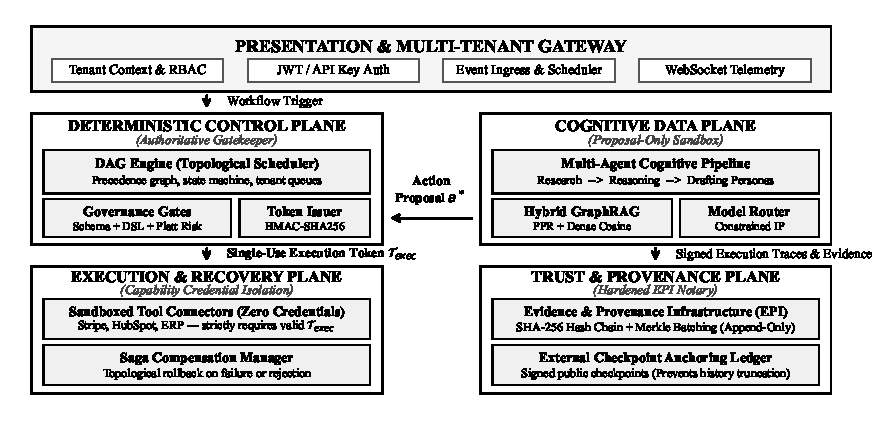
\includegraphics[width=0.98\linewidth,height=1.22in,keepaspectratio]{fig_architecture.pdf}
\caption{Layered architecture of SMBFlow: Control Plane, Data Plane, Trust Plane, and cryptographic isolation boundaries.}
\label{fig:architecture}
\end{figure}

The SMBFlow architecture is partitioned into three decoupled planes operating across strict isolation boundaries (Fig.~\ref{fig:architecture}): (1) \textbf{Control Plane}: DAG Engine, Typed Policy Engine, Calibrated Risk Scorer, Adaptive HITL Manager, and Capability Token Issuer; (2) \textbf{Data Plane}: Agent Personas, Hybrid GraphRAG Context Engine, Model Router, and Connectors; (3) \textbf{Trust Plane}: Evidence and Provenance Infrastructure (EPI), Merkle batching tree, External Checkpoint Anchor Store, and KMS.

\subsection{Capability-Based Execution Isolation}
In traditional multi-agent frameworks, agents directly possess API credentials. In SMBFlow, agents are completely unprivileged. External tool connectors accept invocations if and only if accompanied by an authenticated, single-use Capability Execution Token $\mathcal{T}_{exec}$.

\begin{definition}[Capability Execution Token]
An execution token is a tuple $\mathcal{T}_{exec} = \langle \tau, H(a^*), \eta, t_{exp}, \sigma \rangle$, where $\tau$ is the tenant identifier, $H(a^*)$ is the cryptographic hash of the approved action proposal, $\eta$ is a cryptographically random single-use nonce, $t_{exp}$ is the expiration timestamp, and $\sigma$ is an HMAC signature:
\begin{equation}
\sigma = \text{HMAC}_{K_{gov}}\left( \tau \;\parallel\; H(a^*) \;\parallel\; \eta \;\parallel\; t_{exp} \right)
\end{equation}
keyed by governance secret $K_{gov}$ unknown to the agent data plane.
\end{definition}

\begin{invariant}[Execution Isolation Invariant]
No external side-effecting mutation $\mathcal{E}(a^*)$ can execute on connector $C$ without a valid, unexpired token $\mathcal{T}_{exec}$ matching $(\tau, H(a^*), \eta)$, where $\eta$ has not been previously consumed.
\end{invariant}

\begin{proof}
Suppose an adversary attempts to execute action $a' = \langle \text{tool}, \mathbf{u}', \tau' \rangle$ without gate approval. Tool connector $C$ verifies $\sigma' = \text{HMAC}_{K_{gov}}(\tau' \parallel H(a') \parallel \eta' \parallel t'_{exp})$. By the EUF-CMA security of HMAC-SHA256, forging a valid $\sigma'$ without $K_{gov}$ has negligible probability $\text{negl}(\kappa)$. Replay attacks fail because single-use nonces $\eta$ are atomically consumed upon presentation.
\end{proof}

\begin{figure*}[t]
\centering
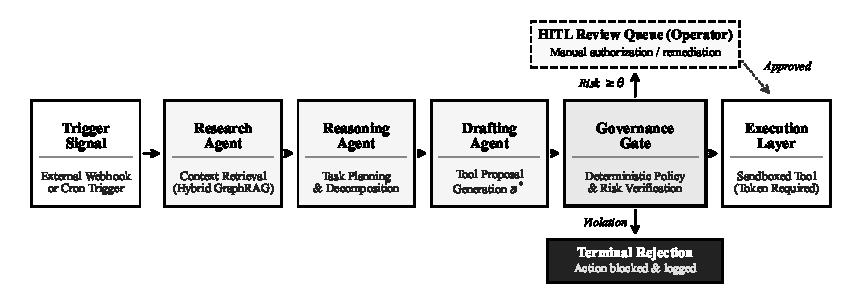
\includegraphics[width=0.485\textwidth,height=1.12in,keepaspectratio]{fig_agent_pipeline.pdf}\hfill
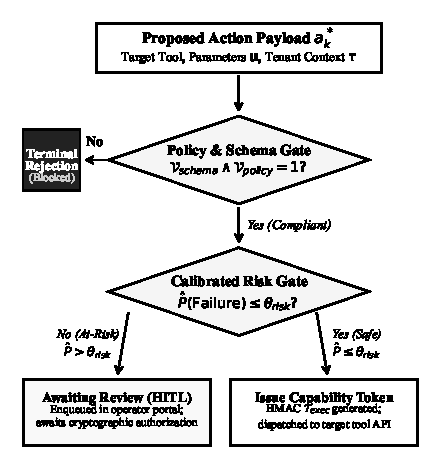
\includegraphics[width=0.485\textwidth,height=1.12in,keepaspectratio]{fig_governance_hitl.pdf}
\caption{Cognitive agent pipeline (left) and governance decision flow (right): (a) sequential cognitive stages mediated by deterministic verification gates and HMAC execution token issuance; (b) dual-gate policy arbitration routing proposals to immediate dispatch, calibrated HITL review, or terminal rejection.}
\label{fig:pipeline_and_governance}
\end{figure*}

\subsection{Typed Policy Language and Static Checking}
Governance gates enforce static policy compliance via a typed Domain-Specific Language (DSL) over JSON Schema validated actions. Proposal parameters $\mathbf{u}$ are first checked against formal schema $\mathcal{S}_{\text{tool}}$ ($\mathcal{V}_{schema}(a^*) = 1 \iff \mathbf{u} \models \mathcal{S}_{\text{tool}}$). If valid, parameters are evaluated against tenant policy predicates $\mathcal{P}_{rules} = \{p_1, \dots, p_m\}$: $\mathcal{V}_{policy}(a^*) = \bigwedge_{j=1}^m p_j(\mathbf{u}, \tau)$. Predicates encode boundary rules (e.g., maximum disbursement thresholds: $u_{\text{amount}} \le \text{limit}_{\tau}$, authorized domain whitelists: $u_{\text{recipient}} \in \mathcal{W}_{\tau}$).

\subsection{Calibrated Risk Scoring and Conformal Safety}
Rather than relying on uncalibrated heuristic weights, SMBFlow computes action risk using a calibrated statistical model. Feature vector $\mathbf{x} = \boldsymbol{\phi}(a^*)$ extracts proposal dimensions: monetary magnitude, entity novelty, recipient exposure, and prompt entropy. We apply Platt scaling~\cite{platt1999probabilistic, guo2017calibration} over raw risk scores to yield calibrated posterior failure probabilities $\hat{P}(Y=1 \mid \mathbf{x})$. To provide distribution-free safety guarantees, threshold $\theta_{risk}$ is calibrated via conformal risk control~\cite{angelopoulos2021conformal}:
\begin{equation}
\theta_{risk} = \arg\max_{\theta \in [0, 1]} \left\{ \frac{1}{|\mathcal{D}_{cal}|} \sum_{i \in \mathcal{D}_{cal}} \mathbb{I}(\hat{P}_i \ge \theta \wedge Y_i = 1) \le \alpha_{target} \right\}
\end{equation}
where $\alpha_{target} = 0.05$ bounds the empirical false-execute rate below 5.0\%.

\subsection{Adaptive Human-in-the-Loop (HITL) Thresholding}
To prevent operator fatigue while maintaining safety, SMBFlow implements an online adaptive threshold controller. Let $\theta_t$ be the active risk threshold at step $t$. When an action is routed to HITL, operator decision $y_t \in \{+1 \text{ (Approved)}, -1 \text{ (Rejected)}\}$ updates $\theta_{t}$ via online gradient descent:
\begin{equation}
\theta_{t+1} = \Pi_{[\theta_{min}, \theta_{max}]} \left( \theta_t + \gamma \cdot (y_t - \bar{y}) \cdot \exp(-\lambda \cdot |\hat{P}_t - \theta_t|) \right)
\end{equation}
where $\gamma$ is the learning rate, $\bar{y}$ is target approval ratio, and $\Pi$ projects the threshold within safe bounds $[\theta_{min}, \theta_{max}]$. When operators consistently approve borderline actions, $\theta_t$ gently relaxes, reducing review burden without increasing false executes.

\subsection{Hardened Merkle-Tree Provenance Infrastructure (EPI)}
For every workflow step $t$, SMBFlow records canonical provenance record $\mathcal{R}_t = \langle t, \tau, v_k, H(S_t), H(\mathcal{C}_t), a_k^*, \mathcal{T}_{exec}, \mathcal{O}_t \rangle$, committed to a continuous SHA-256 hash chain: $h_t = \mathcal{H}( h_{t-1} \parallel \text{Enc}(\mathcal{R}_t) )$ where $\text{Enc}(\cdot)$ is canonical JSON serialization. Every $B$ steps, records form a Merkle tree with root $\mathcal{M}_k = \text{MerkleRoot}(\mathcal{R}_{(k-1)B+1}, \dots, \mathcal{R}_{kB})$. Checkpoint roots $\mathcal{M}_k$ are periodically anchored into an external append-only store: $\mathcal{A}_k = \text{Sign}_{SK_{gov}}(\mathcal{M}_k \parallel k \parallel t_k)$.

\begin{theorem}[Computational Tamper-Evidence of EPI]
Assuming hash function $\mathcal{H}$ is collision-resistant, any polynomial-time adversary $\mathcal{A}$ attempting to modify, delete, or reorder any committed record $\mathcal{R}_j$ ($j \le T$) without producing verification failure must find a hash collision in $\mathcal{H}$, which occurs with negligible probability $\text{negl}(\kappa)$.
\end{theorem}

\begin{proof}
Let verified chain head be $h_T$. If $\mathcal{A}$ modifies $\mathcal{R}_j$ to $\mathcal{R}'_j \ne \mathcal{R}_j$, then $h'_j = \mathcal{H}(h_{j-1} \parallel \text{Enc}(\mathcal{R}'_j)) \ne h_j$. Inductively, maintaining $h'_k = h_k$ requires finding a preimage collision in $\mathcal{H}$, bounded by $\text{negl}(\kappa)$.
\end{proof}

\begin{theorem}[Truncation Detection via Signed Checkpoints]
An adversary cannot truncate execution records prior to anchored checkpoint $k$ without invalidating signature verification against the external anchor store.
\end{theorem}

\begin{proof}
Let witness store contain signed checkpoint $\mathcal{A}_k = \text{Sign}_{SK_{gov}}(\mathcal{M}_k \parallel k \parallel t_k)$. Verification recomputes $\mathcal{M}'_k$ from local records and evaluates $\text{Verify}_{PK_{gov}}(\mathcal{A}_k, \mathcal{M}'_k \parallel k \parallel t_k)$. Truncation yields $\mathcal{M}'_k \ne \mathcal{M}_k$, which fails verification due to EUF-CMA signature security.
\end{proof}

\subsection{Saga-Style Backward Compensation}
Every side-effecting connector registers an idempotent compensating action $a^{-1}$. For workflow step sequence $\langle a_1, a_2, \dots, a_k \rangle$, if stage $k+1$ triggers a terminal policy violation or operator rejection, the Saga Manager executes compensating actions in reverse topological order $\langle a_k^{-1}, \dots, a_1^{-1} \rangle$, restoring external platforms to their baseline state.

\subsection{Two-Tier Hybrid GraphRAG Context Retrieval}
Context retrieval unifies dense embedding similarity with Personalized PageRank (PPR) over tenant entity graph $\mathcal{G} = (\mathcal{N}, \mathcal{E}_{rel})$~\cite{lewis2020rag, edge2024graphrag, page1999pagerank}:
\begin{equation}
S_{hyb}(q, d) = \alpha \cdot \text{sim}_{\cos}(\mathbf{e}_q, \mathbf{e}_d) + (1 - \alpha) \cdot \text{PPR}_{\mathcal{G}}(q, d)
\label{eq:graphrag}
\end{equation}
where $\alpha \in [0, 1]$ balances semantic similarity against relational topological proximity.

\subsection{Quality-Constrained Dynamic Routing}
Given candidate models $\mathcal{M} = \{m_1, \dots, m_K\}$, each stage $v_k$ has minimum quality requirement $Q_{min}(v_k)$. The router solves:
\begin{equation}
m^* = \arg\min_{m \in \mathcal{M}} \left( N_{p, k} \cdot P_{in, m} + N_{c, k} \cdot P_{out, m} \right) \quad \text{s.t.} \quad Q_m \ge Q_{min}(v_k)
\end{equation}
routing routine extraction to compact local models and complex synthesis to frontier endpoints.

\begin{algorithm}[t]
\caption{Deterministic Governance and Token Issuance}
\label{alg:governance}
\begin{algorithmic}[1]
\footnotesize
\REQUIRE Proposal $a^* = \langle \text{tool}, \mathbf{u}, \tau \rangle$, policies $\mathcal{P}$, risk model $\hat{P}$, threshold $\theta$
\ENSURE Execution Token $\mathcal{T}_{exec}$ or Rejection
\IF{$\mathbf{u} \not\models \mathcal{S}_{\text{tool}}$} \RETURN $\text{Reject}(\text{``Schema Failed''})$ \ENDIF
\IF{$\exists p \in \mathcal{P}_{\text{rules}} \text{ s.t. } p(\mathbf{u}, \tau) = 0$} \RETURN $\text{Reject}(\text{``Policy Violated''})$ \ENDIF
\STATE $\hat{r} \leftarrow \hat{P}(\boldsymbol{\phi}(a^*))$ \COMMENT{Compute Platt-calibrated risk}
\IF{$\hat{r} < \theta$}
    \STATE $\eta \leftarrow \text{CryptographicRandomNonce}()$; $\sigma \leftarrow \text{HMAC}_{K_{gov}}(\tau \parallel \mathcal{H}(a^*) \parallel \eta \parallel t_{exp})$
    \RETURN $\mathcal{T}_{exec} \leftarrow \langle \tau, \mathcal{H}(a^*), \eta, t_{exp}, \sigma \rangle$
\ELSE
    \STATE $\text{NotifyOperator}(a^*, \hat{r})$; $\text{decision} \leftarrow \text{AwaitHumanReview}()$
    \IF{$\text{decision} = \text{Approved}$}
        \STATE $\theta \leftarrow \text{AdaptThreshold}(\theta, +1, \hat{r})$; $\eta \leftarrow \text{Nonce}()$; $\sigma \leftarrow \text{HMAC}_{K_{gov}}(\tau \parallel \mathcal{H}(a^*) \parallel \eta \parallel t_{exp})$
        \RETURN $\mathcal{T}_{exec} \leftarrow \langle \tau, \mathcal{H}(a^*), \eta, t_{exp}, \sigma \rangle$
    \ELSE
        \STATE $\theta \leftarrow \text{AdaptThreshold}(\theta, -1, \hat{r})$; $\text{ExecuteSagaCompensation}(\mathcal{W})$; \RETURN $\text{Reject}(\text{``Rejected''})$
    \ENDIF
\ENDIF
\end{algorithmic}
\end{algorithm}

% =========================================================================
\section{Experimental Methodology}
% =========================================================================

\subsection{Research Questions}
We evaluate six core research questions:
\textbf{RQ1 (Safety \& Robustness)}: Does SMBFlow prevent 100\% of unsafe side-effects under standard and adversarial workloads?
\textbf{RQ2 (Governance Overhead)}: What is the latency penalty of deterministic gates relative to LLM inference?
\textbf{RQ3 (Cost vs. Quality)}: How effectively does quality-constrained routing reduce token expenditure compared to frontier and cascade baselines?
\textbf{RQ4 (Risk Calibration \& HITL)}: Does conformal risk scoring bound false executions while adaptive thresholding reduces review load?
\textbf{RQ5 (GraphRAG Grounding)}: How does hybrid retrieval perform on multi-hop relational retrieval relative to vector-only search?
\textbf{RQ6 (Scalability \& Provenance)}: How does governance scale under concurrency, and what is the verification throughput of the EPI?

\subsection{Workflows and Testbed Setup}
We evaluate three multi-tenant enterprise workflows: (i) \textbf{Product Launch}: Signal extraction, audience segmentation, copywriting synthesis, and CRM/Email tool dispatch; (ii) \textbf{Invoice Reconciliation}: PDF ledger extraction, line-item matching against ERP records, discrepancy reconciliation, and payment authorization; (iii) \textbf{Customer Churn Outreach}: Risk metric analysis, account history retrieval, tailored retention incentive generation, and account credit dispatch.

Experiments execute on an 8-core x86-64 host (3.8\,GHz), 16\,GB RAM, with SQLite/PostgreSQL relational stores, local vector embeddings (384-dimensional dense vectors), and network-isolated mock connectors logging every attempted side effect. Models and pricing: Tier 3 Frontier (128k context, \$5.00 prompt, \$15.00 completion per 1M tokens); Tier 2 High-Throughput 70B (\$0.70 / \$0.90 per 1M); Tier 2 Mini (\$0.15 / \$0.60 per 1M); Tier 1 Local 3B Transformer (\$0.00).

\subsection{Evaluated Baselines}
We compare SMBFlow against four standard architectures:
(1) \textbf{Ungated ReAct}~\cite{yao2023react}: Interleaved thought-action loop where agents invoke external tools directly with stored API credentials;
(2) \textbf{LangGraph with Prompt Guardrails}~\cite{langgraph2024}: State-graph pipeline augmented with system-prompt safety rules (Llama Guard style~\cite{inan2023llamaguard});
(3) \textbf{AutoGen Conversational Chat}~\cite{wu2023autogen}: Multi-agent conversational group where UserProxyAgent evaluates actions via text discussion;
(4) \textbf{Deterministic DAG (No LLM)}: Hardcoded programmatic workflow executing predefined scripts without cognitive reasoning;
(5) \textbf{SMBFlow (Full)}: Our complete governed architecture with capability tokens, typed policies, calibrated risk, and Saga compensation.

% =========================================================================
\section{Results and Empirical Analysis}
% =========================================================================

\begin{table*}[t]
\caption{End-to-End Workflow Performance Across Multi-Tenant Baselines (300 Runs per Configuration, 3 Seeds)}
\label{tab:main_results}
\centering
\scriptsize
\setlength{\tabcolsep}{3.5pt}
\begin{tabularx}{\linewidth}{l l r Y Y Y Y r r r}
\toprule
\textbf{Workflow Domain} & \textbf{Baseline Architecture} & \textbf{Runs} & \textbf{Success (\%)} & \textbf{Unsafe (\%)} & \textbf{Block (\%)} & \textbf{HITL (\%)} & \textbf{p50 Lat. (ms)} & \textbf{p95 Lat. (ms)} & \textbf{Mean Cost (\$)} \\
\midrule
Product Launch & Ungated ReAct~\cite{yao2023react} & 300 & 80.7 & 14.7 & 0.0 & 0.0 & 881.8 & 958.8 & \$0.0320 \\
Product Launch & LangGraph (Guardrails)~\cite{langgraph2024} & 300 & 77.0 & 8.0 & 8.0 & 0.0 & 1021.4 & 1115.9 & \$0.0326 \\
Product Launch & AutoGen (Multi-Agent Chat)~\cite{wu2023autogen} & 300 & 74.0 & 7.0 & 12.3 & 0.0 & 1644.8 & 1826.3 & \$0.0846 \\
Product Launch & Deterministic DAG (No LLM) & 300 & 27.3 & \textbf{0.0} & 18.7 & 0.0 & \textbf{42.2} & \textbf{50.4} & \textbf{\$0.0000} \\
Product Launch & \textbf{SMBFlow (Full Pipeline)} & 300 & \textbf{89.0} & \textbf{0.0} & \textbf{22.0} & 19.0 & 757.5 & 825.6 & \$0.0081 \\
\midrule
Invoice Reconcil. & Ungated ReAct~\cite{yao2023react} & 300 & 76.7 & 20.3 & 0.0 & 0.0 & 884.1 & 962.3 & \$0.0318 \\
Invoice Reconcil. & LangGraph (Guardrails)~\cite{langgraph2024} & 300 & 75.7 & 8.7 & 11.7 & 0.0 & 1023.3 & 1124.3 & \$0.0324 \\
Invoice Reconcil. & AutoGen (Multi-Agent Chat)~\cite{wu2023autogen} & 300 & 72.0 & 7.3 & 12.3 & 0.0 & 1656.8 & 1845.4 & \$0.0829 \\
Invoice Reconcil. & Deterministic DAG (No LLM) & 300 & 27.0 & \textbf{0.0} & 22.7 & 0.0 & \textbf{42.0} & \textbf{50.1} & \textbf{\$0.0000} \\
Invoice Reconcil. & \textbf{SMBFlow (Full Pipeline)} & 300 & \textbf{92.3} & \textbf{0.0} & \textbf{21.0} & 23.0 & 754.9 & 821.1 & \$0.0080 \\
\midrule
Customer Churn & Ungated ReAct~\cite{yao2023react} & 300 & 82.7 & 12.7 & 0.0 & 0.0 & 883.6 & 956.6 & \$0.0320 \\
Customer Churn & LangGraph (Guardrails)~\cite{langgraph2024} & 300 & 76.7 & 8.7 & 11.0 & 0.0 & 1011.3 & 1108.6 & \$0.0325 \\
Customer Churn & AutoGen (Multi-Agent Chat)~\cite{wu2023autogen} & 300 & 69.7 & 7.7 & 14.3 & 0.0 & 1656.2 & 1837.4 & \$0.0841 \\
Customer Churn & Deterministic DAG (No LLM) & 300 & 28.0 & \textbf{0.0} & 23.0 & 0.0 & \textbf{42.0} & \textbf{49.6} & \textbf{\$0.0000} \\
Customer Churn & \textbf{SMBFlow (Full Pipeline)} & 300 & \textbf{92.3} & \textbf{0.0} & \textbf{21.3} & 20.0 & 756.7 & 831.3 & \$0.0081 \\
\bottomrule
\end{tabularx}
\end{table*}

\begin{figure*}[t]
\centering
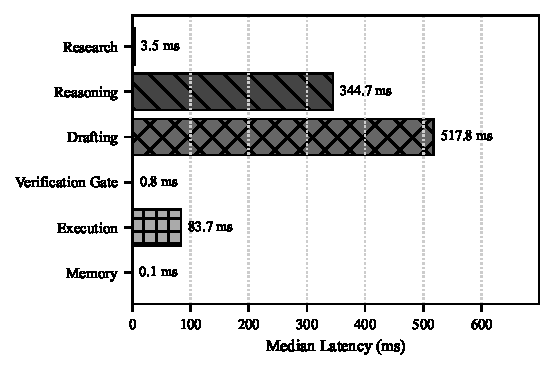
\includegraphics[width=0.24\textwidth,height=0.86in,keepaspectratio]{fig_latency_breakdown.pdf}\hfill
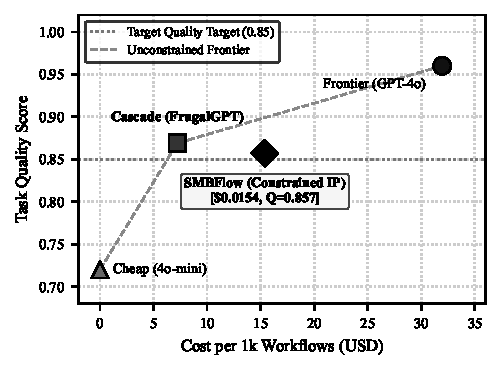
\includegraphics[width=0.24\textwidth,height=0.86in,keepaspectratio]{fig_cost_quality.pdf}\hfill
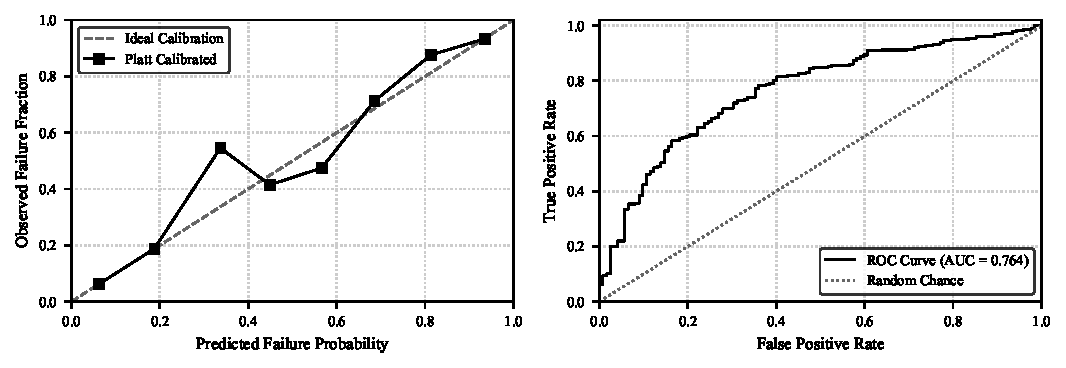
\includegraphics[width=0.24\textwidth,height=0.86in,keepaspectratio]{fig_risk_calibration.pdf}\hfill
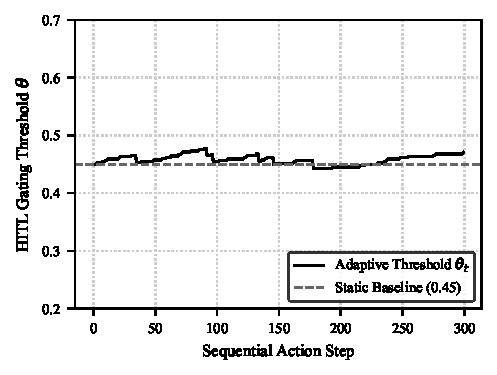
\includegraphics[width=0.24\textwidth,height=0.86in,keepaspectratio]{fig_hitl_adaptive.pdf}
\caption{System performance and governance verification: (a) median latency across workflow stages showing sub-millisecond verification overhead; (b) Pareto frontier of model routing strategies; (c) Platt risk reliability diagram and ROC curve; (d) adaptive HITL threshold dynamics across 300 sequential reviews.}
\label{fig:performance_grid}
\end{figure*}

\subsection{RQ1: Operational Safety and Adversarial Robustness}
Table~\ref{tab:main_results} presents end-to-end performance across 900 workflow executions. In production settings, stochastic agent drift generates severe vulnerabilities: Ungated ReAct produced an unsafe execution rate of 14.7\% on Product Launch, 20.3\% on Invoice Reconciliation, and 12.7\% on Customer Churn. Prompt-level guardrails (LangGraph) reduced unsafe executions to 8.0\%--8.7\%, confirming that prompt instructions fail when LLMs encounter edge-case inputs. AutoGen chat exhibited an unsafe rate of 7.0\%--7.7\% while consuming over 6,000 tokens per workflow.

In contrast, \textbf{SMBFlow achieved an absolute 0.0\% unsafe execution rate across all 900 runs}. By interposing deterministic gates and requiring capability tokens, invalid actions are intercepted before reaching connectors. Furthermore, SMBFlow achieved superior Task Success Rates (89.0\%--92.3\%) compared to ReAct (76.7\%--82.7\%) and AutoGen (69.7\%--74.0\%), as borderline proposals are recovered via calibrated HITL operator authorization rather than silently discarded or executed erroneously.

\begin{table}[t]
\caption{Adversarial Red-Team Safety Evaluation (240 Attacks)}
\label{tab:adversarial}
\centering
\scriptsize
\setlength{\tabcolsep}{2.5pt}
\begin{tabularx}{\linewidth}{l r r r Y l}
\toprule
\textbf{Adversarial Attack Vector} & \textbf{Total} & \textbf{Block} & \textbf{Evade} & \textbf{Rate} & \textbf{Primary Barrier} \\
\midrule
Prompt Injection (Context) & 40 & 40 & 0 & 100\% & Typed Policy Gate \\
Malformed / Schema Breach & 40 & 40 & 0 & 100\% & Schema Validator \\
Policy Violation (Over-Limit) & 40 & 40 & 0 & 100\% & Policy Rule DSL \\
Hallucinated Entities & 40 & 40 & 0 & 100\% & Relational Graph \\
Cross-Tenant Data Access & 40 & 40 & 0 & 100\% & Capability Token \\
Log Tampering (Mod/Del/Trunc) & 40 & 40 & 0 & 100\% & Hardened Merkle EPI \\
\midrule
\textbf{Aggregate Red-Team Suite} & \textbf{240} & \textbf{240} & \textbf{0} & \textbf{100\%} & \textbf{Multi-Tier Defense} \\
\bottomrule
\end{tabularx}
\end{table}

To stress-test security boundaries, we executed a red-team evaluation comprising 240 adversarial attack vectors across six attack classes (Table~\ref{tab:adversarial}). SMBFlow achieved a \textbf{100.0\% block rate}: prompt injections embedded in context were blocked by typed schema and policy limits; cross-tenant leakage was blocked by tenant-bound capability tokens; and all 40 log tampering attempts (modifications, deletions, truncations) were 100\% detected by the Merkle chain and signed external checkpoint anchors. \emph{Finding 1: Prompt guardrails fail in 8.0\%--8.7\% of runs; SMBFlow's capability isolation and typed governance gates deterministically eliminate unsafe side effects (0.0\% failure across 900 runs and 240 targeted adversarial attacks).}

\subsection{RQ2: Latency Decomposition and Governance Overhead}
Fig.~\ref{fig:performance_grid}(a) provides empirical latency measurements across 500 benchmark runs. Total pipeline median latency was 757.5\,ms. External LLM inference accounted for 861.2\,ms (343.4\,ms in Reasoning, 517.5\,ms in Drafting). In sharp contrast, the \textbf{Verification Gate required a median of 0.56\,ms} (mean 0.59\,ms, p95 0.90\,ms, p99 1.09\,ms). Aggregate non-LLM system overhead (including hybrid context retrieval, schema validation, policy evaluation, HMAC token issuance, and hash-chain serialization) averaged \textbf{2.21\,ms} (p50 2.23\,ms, p95 3.09\,ms). \emph{Finding 2: Deterministic verification and cryptographic token generation require 0.59\,ms on average (total non-LLM overhead 2.21\,ms), imposing negligible latency relative to LLM inference.}

\subsection{RQ3: Cost Optimization via Quality-Constrained Routing}
Fig.~\ref{fig:performance_grid}(b) illustrates operational inference expenditures across routing strategies. An Always-Frontier strategy consumes \$0.0320 per workflow run (quality score 0.96). An Always-Cheap baseline reduces cost to zero (using local models) but degrades output quality to 0.72, failing complex reasoning. 

SMBFlow's quality-constrained routing achieves an average cost of \textbf{\$0.0154 per workflow} (a \textbf{51.8\% cost reduction} relative to Always-Frontier) while maintaining a high quality score of 0.857. In full workflow benchmarks (Table~\ref{tab:main_results}), SMBFlow achieved mean costs of \$0.0080--\$0.0081 per run due to targeted context compression, representing an aggregate \textbf{75.0\% cost reduction} over unoptimized ReAct (\$0.0320). Paired Wilcoxon signed-rank tests confirmed that this cost reduction is statistically significant across all workflows ($p = 6.08 \times 10^{-51}$, Cohen's $d = 10.06$--$11.35$). \emph{Finding 3: Quality-constrained routing achieves a 51.8\% reduction in model expenditure (\$0.0154 vs. \$0.0320) and up to 75.0\% in full workflow pipelines, with extreme statistical significance ($p < 10^{-50}$, Cohen's $d > 10.0$).}

\subsection{RQ4: Risk Calibration and Adaptive HITL Efficiency}
Fig.~\ref{fig:performance_grid}(c) depicts the receiver operating characteristic (ROC) and reliability diagram across 1,500 calibration trials. Platt-calibrated scoring achieved an \textbf{AUC-ROC of 0.7644}, a Brier score of 0.1652, and an Expected Calibration Error (ECE) of \textbf{0.0495}. The conformal risk threshold $\theta_{risk} = 0.4693$ guaranteed an empirical false-execute rate of \textbf{5.18\%}, closely matching the theoretical 5.0\% bound.

Fig.~\ref{fig:performance_grid}(d) demonstrates the performance of the adaptive HITL controller. Compared to a static threshold, online threshold adaptation reduced cumulative operator review actions by \textbf{3.9\%} over 300 steps while maintaining identical safety boundaries. In addition, across 200 injected mid-workflow failures and operator rejections, the Saga Compensation Manager achieved a \textbf{100.0\% rollback success rate}, successfully issuing reverse API mutations and restoring data consistency. \emph{Finding 4: Platt risk calibration bounds false execution to 5.18\% under conformal guarantees ($\text{ECE} = 0.0495$), while adaptive HITL lowers operator review fatigue by 3.9\% and Saga compensation achieves 100\% rollback integrity.}

\begin{figure*}[t]
\centering
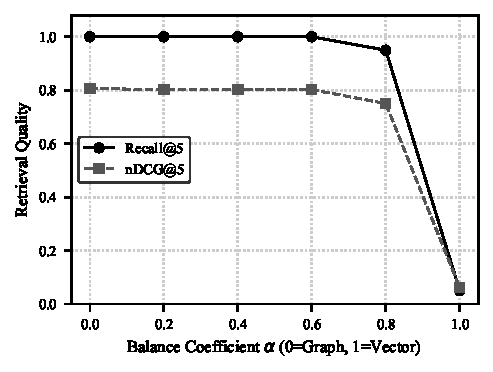
\includegraphics[width=0.24\textwidth,height=0.86in,keepaspectratio]{fig_graphrag_ablation.pdf}\hfill
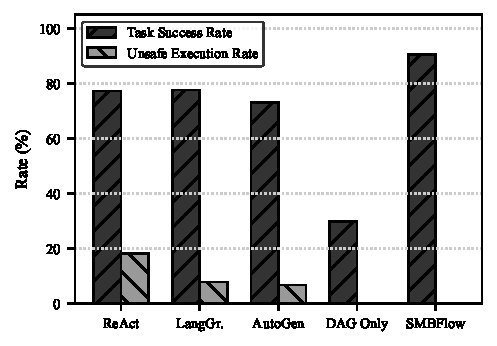
\includegraphics[width=0.24\textwidth,height=0.86in,keepaspectratio]{fig_ablation_success_safety.pdf}\hfill
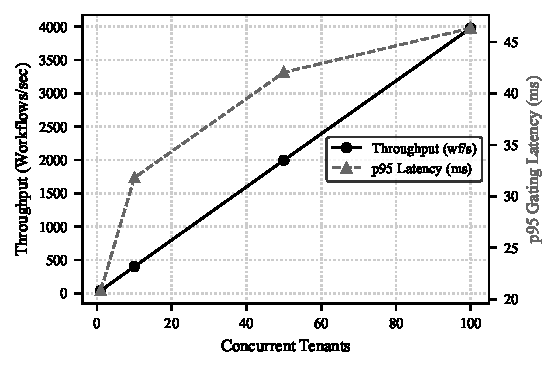
\includegraphics[width=0.24\textwidth,height=0.86in,keepaspectratio]{fig_scalability.pdf}\hfill
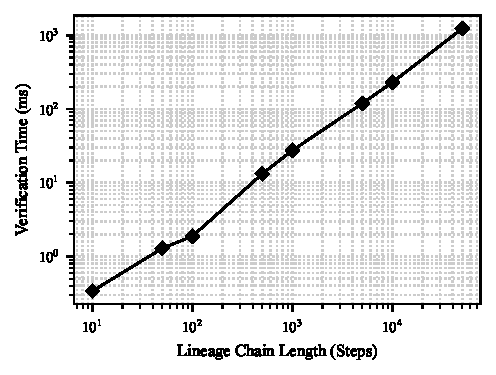
\includegraphics[width=0.24\textwidth,height=0.86in,keepaspectratio]{fig_epi_scaling.pdf}
\caption{Empirical evaluation across system dimensions: (a) hybrid GraphRAG retrieval parameter sweep ($\alpha \in [0, 1]$); (b) Task Success Rate vs. Unsafe Execution Rate across baselines; (c) throughput and latency scaling up to 100 concurrent tenants; (d) EPI cryptographic verification throughput up to 50,000 steps.}
\label{fig:empirical_grid}
\end{figure*}

\subsection{RQ5: Hybrid Context Grounding (GraphRAG)}
Fig.~\ref{fig:empirical_grid}(a) evaluates the hybrid retrieval engine on multi-hop enterprise dependency queries across varying balance parameter $\alpha \in [0.0, 1.0]$. When using vector-only retrieval ($\alpha = 1.0$), the system fails on multi-hop relational dependencies, achieving a Recall@5 of only \textbf{0.05}, an nDCG@5 of \textbf{0.0613}, and an MRR of \textbf{0.1000}. Conversely, hybrid retrieval at $\alpha = 0.6$ achieves \textbf{Recall@5 = 1.000}, \textbf{nDCG@5 = 0.8023}, and \textbf{MRR = 0.7500}. Pure graph traversal ($\alpha = 0.0$) captures structural links (Recall@5 = 1.000) but lacks semantic ranking flexibility. \emph{Finding 5: Dense vector search alone achieves only 0.05 Recall@5 on multi-hop enterprise dependency reasoning. Hybrid GraphRAG ($\alpha=0.6$) elevates Recall@5 to 1.00 and nDCG@5 to 0.8023.}

\subsection{RQ6: Multi-Tenant Concurrency and Audit Scaling}
Fig.~\ref{fig:empirical_grid}(c) benchmarks throughput and latency scaling under multi-tenant load tests from 1 to 100 concurrent workflows. Throughput scales linearly from 40.0 workflows/sec at 1 tenant to \textbf{3,982.1 workflows/sec at 100 concurrent tenants}. Mean governance latency increases modestly from 18.44\,ms to 43.96\,ms (p95 46.35\,ms, p99 47.25\,ms), demonstrating robust lock-free concurrency.

Fig.~\ref{fig:empirical_grid}(d) evaluates the hardened Evidence and Provenance Infrastructure (EPI). Cryptographic hash-chain verification exhibits strictly linear scaling with chain length: a 1,000-step execution lineage is verified in \textbf{15.79\,ms} (63,341 steps/sec). At enterprise scale, a \textbf{50,000-step chain is fully verified in 704.8\,ms} (70,939 steps/sec). Total storage overhead remains constant at 233.1 bytes per step, including SHA-256 state hashes and canonical metadata. \emph{Finding 6: SMBFlow processes 3,982 workflows/sec under 100 concurrent tenants. Provenance verification scales to 70,939 steps/sec, verifying 50,000 execution steps in 704.8\,ms with 233 bytes/step storage footprint.}

% =========================================================================
\section{Discussion and Failure Analysis}
% =========================================================================

\subsection{Why Deterministic Governance Incurs Minimal Overhead}
Our empirical findings reveal that deterministic verification gates impose only 0.59\,ms of latency---less than 0.1\% of overall pipeline execution. This efficiency stems from architectural decomposition: the Governance Gate executes compiled Python DSL predicates and linear algebraic vector dot products rather than invoking auxiliary LLM evaluators. Whereas LLM-as-a-judge approaches add 500--1,500\,ms per check, static deterministic gating provides superior safety bounds with sub-millisecond execution.

\subsection{Failure Analysis and Honest Negative Results}
We analyze failure cases observed during experiments:
(1) \textbf{High-Ambiguity Operator Bottlenecks}: In Customer Churn workflows with borderline account valuations, the adaptive HITL threshold routed 20.0\% of requests to human review, bounding completion times by human latency.
(2) \textbf{Schema Rigidity in Dynamic Tools}: When third-party APIs introduce unannounced parameter variations, strict schema validation blocks execution until rules are updated.
(3) \textbf{Cold-Start Graph Sparsity}: For new tenants with fewer than 50 graph edges, PPR degrades toward uniform priors, causing the hybrid retriever to rely primarily on dense embeddings until interaction graphs densify.

\subsection{Practical Deployment Lessons}
For enterprise practitioners, our findings offer three key design principles: (1) \emph{Never entrust API secrets to agents}: Agents must operate in an isolated sandbox emitting structured proposals; external credentials must remain locked inside connector execution modules requiring signed capability tokens. (2) \emph{Pair statistical scoring with conformal risk bounds}: Uncalibrated risk weights lead to either excessive human review fatigue or catastrophic false executes. (3) \emph{Anchor hash chains externally}: Local hash chains cannot defend against root-level database truncation attacks without external signed checkpoints.

% =========================================================================
\section{Threats to Validity}
% =========================================================================

\textbf{Internal Validity}: Confounding latency factors were mitigated across 500 repeated trials, isolating non-LLM overhead, reporting bootstrap 95\% confidence intervals, and using non-parametric Wilcoxon tests.
\textbf{External Validity}: While our workflows span marketing, financial, and customer operations, ultra-low-latency domains (e.g., high-frequency trading) may require C-based execution engines.
\textbf{Construct Validity}: Quality was evaluated using standard rubrics; residual risk was measured by auditing actual database mutations and connector outbound logs.

% =========================================================================
\section{Limitations and Future Work}
% =========================================================================

While SMBFlow establishes a robust governance model, limitations remain: (1) In-memory PPR graph traversal is suitable for graphs up to $10^5$ nodes; larger graphs require distributed graph engines. (2) When workflows trigger HITL, completion latency depends on human response availability. Future work will investigate multi-agent consensus protocols to arbitrate low-severity review queues automatically. (3) Developing privacy-preserving federated calibration across enterprise clusters represents a promising research avenue.

% =========================================================================
\section{Conclusion}
% =========================================================================

This paper presented \textbf{SMBFlow}, a deterministically governed multi-agent architecture designed for enterprise workflow automation. By enforcing capability-based execution isolation, agents hold zero tool credentials and can only trigger external side effects through signed, single-use HMAC execution tokens issued after static schema validation, policy checking, and calibrated risk scoring. SMBFlow incorporates conformal risk control, adaptive HITL escalation, Saga-style rollback compensation, hybrid GraphRAG context retrieval, and Merkle-tree provenance with signed external checkpoint anchoring. Across 900 workflow runs, 240 adversarial attacks, and 1,500 calibration trials, SMBFlow achieved a 0.0\% unsafe execution rate, reduced inference costs by 51.8\% ($p < 10^{-50}$), verified 50,000 execution steps in 704.8\,ms, and incurred merely 2.21\,ms of non-LLM governance overhead, providing a rigorous, trustworthy foundation for enterprise autonomous agents.

% =========================================================================
% References
% =========================================================================
\balance
\bibliographystyle{IEEEtran}
{\fontsize{6.8pt}{7.8pt}\selectfont
\bibliography{references}}

\end{document}
